% !TEX root = ../../main.tex
\section{One-Class Classification}\label{sec:one_class_classification}
As discussed in the previous section, change detection in time series can be implemented using outlier, or novelty, detection.
To regard a data point as an outlier, there must be a model of the normal time series data and a (dis)similiarity measure defined over the model and data objects.
When a data point differs enough from the created model, it can be labeled as an outlier.
The class of \gls{occ} algorithms is especially designed for that purpose.
The algorithms build up a model of the data, assuming only normal data objects are available (or a very limited amount of example outlier data objects).
This is also known as novelty detection or semi-supervised detection and is of Type 3 in the system by Hodge and Austin~\cite{hodge2004survey}.
This differs from classical classification algorithms, which commonly rely of both positive and negative examples.

In \Cref{subsec:occ-problem-formulation} the problem formulation of \gls{occ} methods is explained.
In \cref{subsec:occ-methods} an overview of \gls{occ} methods is given.
The following section will discuss one specific set of methods, the \gls{oc-svm} which use \glspl{svm} to model the normal training data.

\subsection{Problem formulation}\label{subsec:occ-problem-formulation}
The problem of \acrlong{occ} is closely related to the (traditional) two-class classification situation\footnote{Two-class problems are considered the basic problem, since multi-class classification problems can be decomposed into multiple two-class problems \cite{fukunaga1990introduction}.}.
In the case of traditional classification algorithms, the problem is to assign an unknown object to one of the pre-defined categories.
Every object $i$ is represented as a d-dimensional vector $\vectorsym{x}_i = (x_{i,1},\dots,x_{i,d}), x_{i,j} \in \mathbb{R}$.
Using this notation, an object $\vectorsym{x}_i$ thus represents one point in a feature space $\mathcal{X} \in \mathbb{R}^d$.
The two classes of objects, $\omega_1$ and $\omega_2$, are labeled $-1$ and $+1$ respectively.
The objects with a label $y_i \in \{-1, +1\}$ are in the training set (note that it can be both positive and negative example objects).
This problem is solved by determining a decision boundary in the feature space of the data objects and label the new data object based on the location relative to this boundary.
This is expressed by the decision function $y = f(\vectorsym{x})$:
\begin{equation}\label{eq:decision_function_classification}
  f: \mathbb{R}^d \rightarrow \{-1, +1\}
\end{equation}
In case of the \gls{occ} problem, only one class (often referred as the target class, or positive examples) of training data is used to create a decision boundary.
The goal is to determine whether a new data object belongs to the target class.
If it does not belong to the class it is an outlier.
One could argue that this problem is equal to the traditional two-class problem by considering all other classes as negative examples, although there are important differences.
In pure \gls{occ} problems there are no negative example objects available.
This could be because the acquisition of these examples is very expensive, or because there are only examples of the `normal' state of the system and the goal is to detect `abnormal' states.
Since the algorithm's goal is to differentiate between normal and abnormal objects (relative to the training objects), \gls{occ} is often called outlier, novelty or anomaly detection, depending on the origin of the problem to which the algorithm is applied\footnote{The term \acrlong{occ} originates from Moya \etal \cite{moya1993one}.}.
The difference between two and one-class classification and the consequence for outlier objects is illustrated in \Cref{fig:two-vs-one-classification}.
In the two-class classification problem the object \textbf{o} will be member of the \textbf{-1} class whilst the \gls{occ} problem will label it as an outlier.
In \cite{tax2001one} a more detailed analysis of the \gls{occ} is given.

\begin{figure}
  \centering
    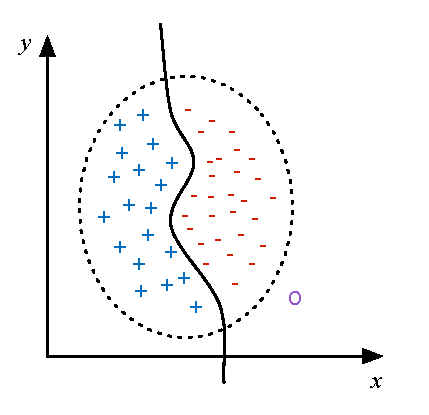
\includegraphics[width=0.5\textwidth,keepaspectratio]{./Figures/chapter3/two-vs-one-classification.pdf}
  \caption[Difference between two and one-class classification]{This plot shows the difference between two and one-class classification. The solid line indicates a possible decision boundary between the \textbf{+1} and \textbf{-1} example objects. The dashed circle indicates the closed boundary around all the data objects. In the first type the object \textbf{o} is considered to be member of the \textbf{-1}-class, whilst in the latter (\gls{occ}) formulation it is an outlier.}
  \label{fig:two-vs-one-classification}
\end{figure}

The \gls{occ} algorithms have been applied to a wide range of applications.
The first is, obviously, outlier detection of objects which do not resemble the bulk of the training data.
It can be a goal by itself and can be used as a filtering mechanism for other data processing methods.
Often methods that rely on data characteristics are sensitive for remote regions in the data set.
Using \gls{occ} these remote regions can be removed from the data set.
A second application is for the problem as described above, in which only data from a single target class is available.
When this problems originates from \eg a monitoring process, the \gls{occ} is able to recognize abnormal system states, without the need to create (or simulate) faulty states beforehand.
The final possible application given by Tax \cite{tax2001one} is the comparison of two data sets.
By constructing a \gls{occ}-classifier using a training data set, one can compare that set to a new data set.
This will result in a similarity measure expressed in the properties of outliers.
This is related to other methods of expressing similarity, such as density-ratio estimation and the \gls{kl} divergence as discussed in \Cref{sec:change_detection_time_series}.

\subsection{One-Class Classification methods}\label{subsec:occ-methods}
The methods and algorithms used for the \gls{occ}-problem can be organized into three categories \cite{tax2001one,noumir2012simple}, visually represented in \Cref{fig:occ-methods}.
The first category consists of methods that estimate the density of the training data and set a threshold on this density.
Among those are Gaussian models, \glspl{gmm} and Parzen density estimators.
In order to get good generalization results with these methods, the dimensionality of the data and the complexity of the density need to be restricted.
This can cause a large bias on the data.
When a good probability model is postulated, these methods work very well. %, since when one threshold is optimized, a minimum volume is automatically found for the given probability density model \cite{tax2001one}.

Boundary methods are based on Vapnik's principle\footnote{With a limited amount of data available, one should avoid solving a more general problem as an intermediate step to solve the original problem \cite{vapnik1998statistical}.} which imply in this case that estimating the complete data density for a \gls{occ} may be too complex, if one is only interested in the closed boundary.
Examples of methods that focus on the boundary (a direct threshold) of the training data distribution are K-centers, Nearest-neighborhood, and \gls{svdd}, or a combination of those methods \cite{hempstalk2008one}.
Especially \gls{svdd} has a strong bias towards minimal volume solutions.
These type of methods are sensitive to the scale and range of features, since they rely on a well-defined distance measure.
The number of objects that is required, is smaller than in the case of density methods.
The boundary method \gls{svdd}, constructed by Tax and which has shown good performance \cite{khan2010survey}, will be further discussed in \Cref{subsec:oc-svm-svdd}.

Reconstruction methods take a different approach.
Instead of focusing on classification of the data and thus on the discriminating features of data objects, they model the data.
This results in a compact representation of the target data and for any object a reconstruction error can be defined.
Outliers are data objects with a high error, since they are not well reconstructed by the model.
Examples of reconstruction methods are K-means, \gls{pca} and different kind of neural network implementations.

\begin{figure}
  \centering
    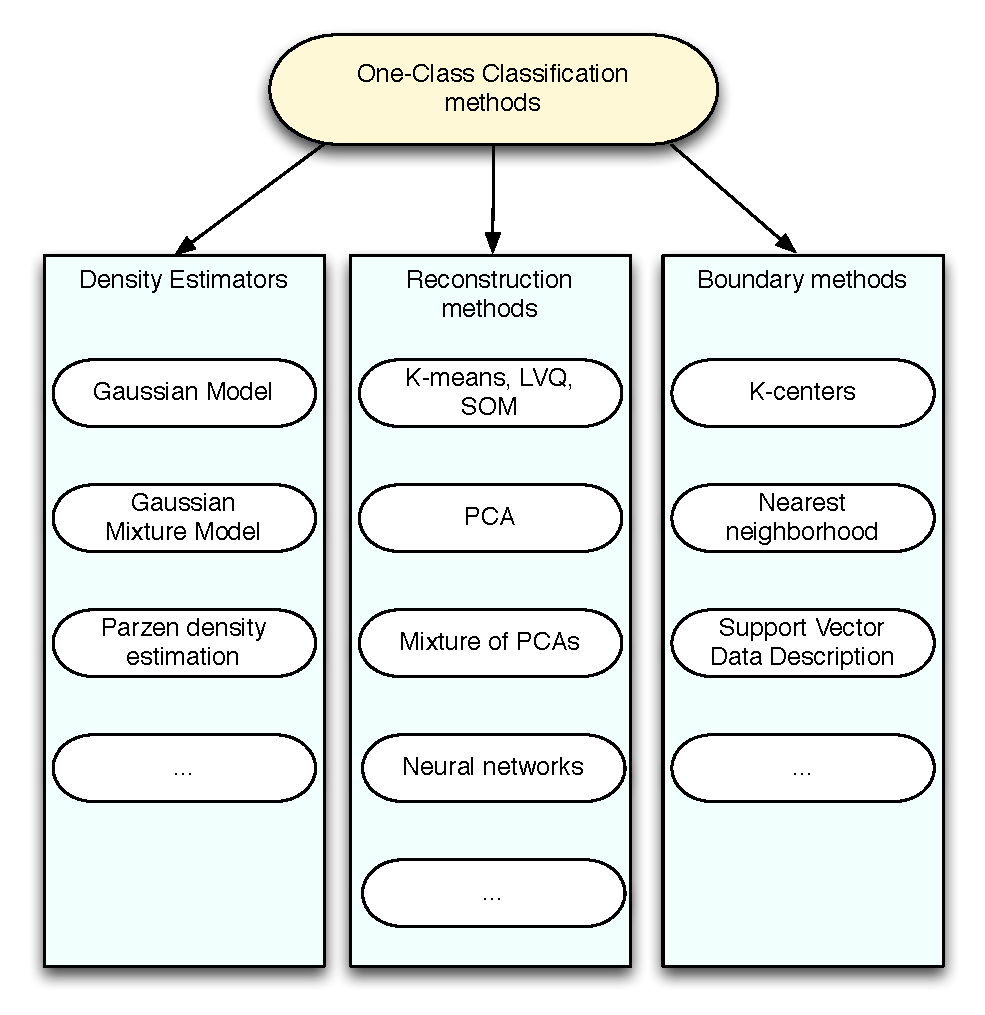
\includegraphics[width=0.5\textwidth,keepaspectratio]{./Figures/chapter3/occ_methods.pdf}
  \caption[One-Class Classification methods]{Overview of \gls{occ} methods categorized in Density Estimation, Reconstruction methods, and Boundary methods. This categorization follows the definition of Tax in \cite{tax2001one}.}
  \label{fig:occ-methods}
\end{figure}

In \cite{khan2010survey,noumir2012simple} an overview of applications for \gls{occ}-algorithms, and explictly for \gls{svm}-based methods (such as \gls{svdd} and \gls{nu-svm}), is given.
It shows succesful applications for, amonst others, problems in the field of Handwritten Digit Recognition, Face Recognition Applications, Spam Detection and Anomaly Detection \cite{li2003improving,perdisci2006using}.
As discussed in \Cref{sec:change_detection_time_series}, this can be used for change detection in time series data.

In this Section we have discussed the problem of \gls{occ} and different kind of implementations.
An often used implementation is the \gls{svm}-based method \cite{noumir2012simple}, since is shows good performance in comparitive researches \cite{khan2010survey,smola1998connection}.
In the following section (\ref{sec:one_class_svm}) two implementations of \gls{oc-svm} will be discussed, the \gls{svdd} method of Tax and Duin \cite{tax1999support} and the \gls{nu-svm}-algoritm by Sch\"olkopf.

% -- Literature --

% ``A survey of recent trends in one class classification'' \cite{khan2010survey}. 25, 2010 \\

% ``One-class classification by combining density and class probability estimation'' \cite{hempstalk2008one}. 51, 2008 \\

% ``One-class classification'' \cite{tax2001one}. 693, 2001 \\

% ``The One-Class Classification Approach to Data Description and to Models Applicability Domain'' \cite{baskin2010one}. 19, 2009 \\

% ``One-class classifier networks for target recognition applications'' \cite{moya1993one}. 70, 1993. Origin of term ``One-Class Classification'' \\